\documentclass[10pt,journal,compsoc]{IEEEtran}

\usepackage[utf8]{inputenc}
\usepackage[spanish,es-tabla]{babel}
\usepackage[noadjust]{cite}
%\usepackage{cite}
\usepackage[pdftex]{graphicx}
\usepackage{amsmath}
\usepackage{acronym}
\usepackage{algorithmic}
\usepackage[linesnumbered,ruled,vlined]{algorithm2e}
\usepackage{array}
\usepackage{mdwmath}
\usepackage{natbib}
%%\usepackage[backend=biber,style=alphabetic,sorting=ynt]{biblatex}
%\addbibresource{bi.bib}

\usepackage{mdwtab}
\usepackage{eqparbox}
\ifCLASSOPTIONcompsoc
  \usepackage[caption=false,font=footnotesize,labelfont=sf,textfont=sf]{subfig}
\else
  \usepackage[caption=false,font=footnotesize]{subfig}
\fi
\usepackage{fixltx2e}
\usepackage{stfloats}
\usepackage{url}
\usepackage[pdftex]{thumbpdf}
\usepackage{minted}

\usepackage{supertabular,booktabs}

\renewcommand{\baselinestretch}{1.05}


\usepackage{lineno}
\linenumbers
\setlength\columnsep{25pt}


\usepackage{listingsutf8}
\lstset{
inputencoding=utf8/latin1,
upquote=true,
  basicstyle=\small,
  breaklines=true,
  keywordstyle=\color{black}\bfseries\em,
  keywords={,input, output, return, datatype, function, in, if, else, foreach, while, begin, end, } %add the keywords you want, or load a language as Rubens explains in his comment above.
  }

\newcommand\MYhyperrefoptions{bookmarks=true,bookmarksnumbered=true,
pdfpagemode={UseOutlines},plainpages=false,pdfpagelabels=true,
colorlinks=true,linkcolor={black},citecolor={black},urlcolor={black},
pdftitle={Bare Demo of IEEEtran.cls for Computer Society Journals},%<!CHANGE!
pdfsubject={Typesetting},%<!CHANGE!
pdfauthor={Michael D. Shell},%<!CHANGE!
pdfkeywords={Computer Society, IEEEtran, journal, LaTeX, paper,
             template}}%<^!CHANGE!


\hyphenation{op-tical net-works semi-conduc-tor}
\begin{document}
\title{Multiplicación Rusa para números grandes}

\author{ Sergio~Salinas,
        Danilo~Abellá}

\markboth{Metodología de investigación, Licenciatura en ciencia de la computación, DMCC, USACH - 16 de noviembre 2017 }%
{Shell \MakeLowercase{\textit{et al.}}: Bare Advanced Demo of IEEEtran.cls for IEEE Computer Society Journals}

\IEEEtitleabstractindextext{%
\begin{abstract}
Dado que en la codificación de algoritmos de multiplicación convencional se utilizan variables numéricas para guardar los factores y el producto, esto termina limitando el tamaño máximo de dígitos que se pueden utilizar para representar un número debido al uso limitado de memoria.
Para poder llevar a cabo una multiplicación de números gigantes se propone utilizar el algoritmo de la multiplicación rusa, en el cual guardando los factores y el producto en cadenas de caracteres y utilizando memoria dinámica, se va operando carácter por carácter hasta finalizar la operación, haciendo uso de los clásicos métodos de suma, división y multiplicación en el proceso.
\end{abstract}


\begin{IEEEkeywords}
Multiplicación Rusa, Números grandes, C.
\end{IEEEkeywords}}


\maketitle

\IEEEdisplaynontitleabstractindextext
\IEEEpeerreviewmaketitle


\ifCLASSOPTIONcompsoc
\IEEEraisesectionheading{\section{Introduction}\label{sec:introduction}}
\else
\section{w}
\label{sec:introduction}
\fi
\IEEEPARstart{E}{}l sistema de multiplicación aprendido en la educación básica es el más habitual a nivel mundial desde que se extendió la numeración arábiga (el sistema decimal que es utiliza actualmente), sin embargo hay otros muchos métodos o estrategias para obtener el resultado de una multiplicación, ya sea de forma mas eficiente o accesible a la hora de programar.
\\\\
Desde hace muchos siglos las matemáticas han sido un punto fuerte en países como Rusia y del Norte de Europa, logrando así un éxito muy considerable al lograr aportar métodos muy interesantes para la multiplicación [\cite{RM06}].
Uno de los más conocidos es el llamado método de los campesinos rusos (o simplemente, multiplicación rusa), un sistema que podemos definir como “lento pero seguro”. De las características mas importantes a destacar se tiene que los únicos conocimientos requeridos son saber sumar, así como dividir y multiplicar por dos, sin saber ninguna otra tabla de multiplicación, por lo que brinda una perspectiva muy diferente a la hora de operar.
\\\\
El tema a analizar en este informe es la efectividad del algoritmo del método de la multiplicación rusa para multiplicar números gigantes que no pueden ser utilizados en algoritmos de multiplicación mas convencionales, por falta de memoria.

\section{¿Qué es la Multiplicación?}

La multiplicación consiste en una operación de composición que requiere sumar reiteradamente un número de acuerdo a la cantidad de veces indicada por otro, o sea, una suma abreviada de sumandos iguales, que pueden repetirse muchas veces [\cite{KPR86}].

\begin{center}
\[
\begin{array}{rl l}
& 2 \hspace{0.2cm} x \hspace{0.2cm} 4 \hspace{0.2cm} = \hspace{0.2cm} 2 \hspace{0.2cm} + \hspace{0.2cm} 2 \hspace{0.2cm} + \hspace{0.2cm} 2 \hspace{0.2cm} + \hspace{0.2cm} 2 \hspace{0.2cm} = \hspace{0.2cm} 8\\
\end{array}
\]
\end{center}

El significado de su palabra lo dice todo, la cual es originada del latín “multus” que corresponde a mucho, y “plico”, que es doblar.
\\\\
Los números que forman parte del proceso de la multiplicación reciben el nombre de factores, mientras que el resultado se denomina producto. Por lo tanto, el objetivo de la operación es hallar el producto de dos factores.
Cada factor, por otra parte, tiene su propia denominación. La cifra a sumar repetidamente es el multiplicando, mientras que el número que indica la cantidad de veces que hay que sumar el multiplicando es el multiplicador. La multiplicación, en definitiva, consiste en tomar el multiplicando y sumarlo tantas veces como unidades contiene el multiplicador para obtener un producto [\cite{KPR86}].

\begin{center}
\[
\begin{array}{rl l}
&  \hspace{-1cm} multiplicando \hspace{4.2cm} producto \\
& \downarrow \hspace{5.7cm} \downarrow \\
& 2 \hspace{0.2cm} x \hspace{0.2cm} 4 \hspace{0.2cm} = \hspace{0.2cm} 2 \hspace{0.2cm} + \hspace{0.2cm} 2 \hspace{0.2cm} + \hspace{0.2cm} 2 \hspace{0.2cm} + \hspace{0.2cm} 2 \hspace{0.2cm} = \hspace{0.2cm} 8 \\
& \hspace{0.8cm} \uparrow \\
& multiplicador \\
\end{array}
\]
\end{center}

Como se puede ver en el ejemplo la multiplicación, 2 x 4 es lo mismo que sumar 2 cuatro veces, dando en ambos casos el 8 como producto.
\\\\
La multiplicación cumple cuatro propiedades que harán más fácil la resolución de problemas. Estas son las propiedades conmutativa, asociativa, elemento neutro y distributiva [\cite{AS00}].
\\\\
La propiedad conmutativa dice que cuando se multiplican dos números, el producto es el mismo sin importar el orden de los multiplicandos.

\begin{center}
\[
\begin{array}{rl l}
&  \hspace{-1cm} multiplicando \hspace{1.8cm} producto \\
& \downarrow \hspace{3.25cm} \downarrow \\
& 2 \hspace{0.2cm} x \hspace{0.2cm} 4 \hspace{0.2cm} = 4 \hspace{0.2cm} x \hspace{0.2cm} 2 \hspace{0.2cm} = \hspace{0.2cm} 8 \\
& \hspace{0.8cm} \uparrow \\
& multiplicador \\
\end{array}
\]
\end{center}

Como se muestra en el ejemplo, el producto de la multiplicación siempre será 8 independiente de si el 2 o 4 son multiplicando o multiplicador respectivamente.
\\\\
Para la propiedad asociativa se afirma que cuando se multiplican tres o más números, el producto es el mismo sin importar como se agrupan los factores.

\begin{center}
\[
\begin{array}{rl l}
& 2 \hspace{0.2cm} x \hspace{0.2cm} ( \hspace{0.2cm} 4 \hspace{0.2cm} x \hspace{0.2cm} 3 \hspace{0.2cm} ) \hspace{0.2cm} = \hspace{0.2cm} ( \hspace{0.2cm} 2 \hspace{0.2cm} x \hspace{0.2cm} 4 \hspace{0.2cm} ) \hspace{0.2cm} x \hspace{0.2cm} 3 \hspace{0.2cm} = \hspace{0.2cm} 24 \\
\end{array}
\]
\end{center}

En este ejemplo se muestra que el producto de multiplicar el resultado de 4 x 3 por 2, es exactamente el mismo que el de multiplicar el resultado de 2 x 4 por 3, en ambos casos da 24.
\\\\
Luego se tiene la propiedad del elemento neutro que dice que el producto de cualquier número por uno es el mismo número.

\begin{center}
\[
\begin{array}{rl l}
& \hspace{0.15cm} elemento \\
& \hspace{0.35cm} neutro \\
& \hspace{0.775cm} \downarrow \\
& 4 \hspace{0.2cm} x \hspace{0.2cm} 1 \hspace{0.2cm} = \hspace{0.2cm} 4 \\
\end{array}
\]
\end{center}

En el ejemplo se muestra el 4 como multiplicando y el 1 como multiplicador, el cual al ser este último el elemento neutro, da 4 como producto.
\\\\
Finalmente tenemos la propiedad distributiva que dice que la suma de dos números por un tercero es igual a la suma de cada sumando por el tercer número.

\begin{center}
\[
\begin{array}{rl l}
& 2 \hspace{0.2cm} x \hspace{0.2cm} ( 6 \hspace{0.2cm} + \hspace{0.2cm} 4 \hspace{0.2cm} ) \hspace{0.2cm} = \hspace{0.2cm} 2 \hspace{0.2cm} x \hspace{0.2cm} 6 \hspace{0.2cm} + \hspace{0.2cm} 2 \hspace{0.2cm} x \hspace{0.2cm} 4 \hspace{0.2cm} = \hspace{0.2cm} 20 \\
\end{array}
\]
\end{center}

El multiplicar la suma de 6 + 4 (o sea 10) por 2 da exactamente el mismo resultado que sumar la multiplicación de 2 x 6 mas 2 x 4, siempre dará 20 como resultado.
\\\\

\section{La multiplicación rusa}

Es un método de multiplicación basado en la forma en que multiplicaban los campesinos rusos en el siglo XIX [\cite{DP06}], el método esta basado en duplicar  y reducir números a la mitad, también se le llama multiplicación binaria debido a que su lógica esta basada la forma binaria de los números

Sean $n$ y $m$ dos números enteros positivos de los que se quiere conocer su producto, se puede computar el resultado usando el método de la multiplicación rusa o multiplicación binaria, este método divide constantemente el primer número por 2 y multiplica constantemente el segundo número por 2 [\cite{AL14}].

	El método se puede expresar mediante las dos siguientes formulas.

Si $n$ es par

$$ n \cdot m  = \dfrac{n}{2} \cdot 2m $$

Si $n$ es impar

$$ n \cdot m  = \dfrac{n-1}{2} \cdot 2m + m$$

Estas formulas tienen como caso trivial cuando $1 \cdot m = m$ para parar. Con ellas se puede calcular el producto de $n \cdot m$ recursivamente o iterativamente. En la tabla \ref{tab:eje1} se muestra un ejemplo de multiplicar 121*35 usando este método.

\begin{table}[!h]
\centering
\label{tab:eje1}
\begin{tabular}{ll|l}
n   & m    & Sumar \\ \hline
121 & 35   & 35    \\
60  & 70   &       \\
30  & 140  &       \\
15  & 280  & 280   \\
7   & 560  & 560   \\
3   & 1120 & 1120  \\
1   & 2240 & 2240  \\ \hline
    &      & 4235
\end{tabular}
\caption{Multiplicación de $121\cdot 35$}
\end{table}

El pseudocódigo de la versión iterativa se muestra en el algoritmo \ref{alg:mrite}, en la linea 6 se aprecia que se puede mezclar la división de las dos formulas en una usando la función piso que aproxima el resultado de la división por dos al menor entero, aun así se sigue teniendo el caso de cuando a es impar ya que este caso dice cuando hay que sumar b al resultado.


\begin{algorithm}
\DontPrintSemicolon
\KwData{Dos enteros positivos a y b}
\KwResult{El resultado del producto de a y b.}
\Begin{
$res \leftarrow 0$\;
\While{$a>0$}{
	\If{a is impar}{
    	res $\leftarrow$ res + b\;
    }
    a $\leftarrow$ $\left\lfloor \dfrac{a}{2} \right\rfloor$ \;
    b $\leftarrow$ $ 2 \cdot b $ \;
    }
    \Return{res}  \;
}
\caption{ Multiplicación rusa}
\label{alg:mrite}
\end{algorithm}

La multiplicación rusa funciona debido a que la multiplicación es distributiva [\cite{DP06}], por ejemplo.

\begin{align}
12 \cdot 9 & = 12 \cdot (1\cdot 2^0 +  0\cdot 2^1 + 0\cdot 2^2 +1\cdot 2^3) \\
& = (12\cdot 2^0 +  0\cdot 2^1 + 0\cdot 2^2 +12 \cdot 2^3) \\
& = 12 + 96 \\
& = 108.
\end{align}

Al proceso de multiplicar repetidamente un número por dos se le llama dubling y al de dividir continuamente por dos halving [\cite{DP06}].

La multiplicación rusa usa el proceso de halving para convertir el primer número a multiplicar en binario y la técnica de dubling que es la que simula el $2^n$ en el ejemplo, de esta forma multiplica dos números convirtiendo el primer número en sumas de factores de dos y multiplicando el  segundo número por esos factores y sumando todos los factores de dos que no estén siendo multiplicados por cero, que es cuando hay un 1 en su expresión binaria. 

La tabla \ref{tab:eje2} hace un paralelo entre la multiplicación rusa con los números en su forma decimal y binaria, con esta tabla se puede ver la relación que tiene multiplicación rusa con los números binarios ya que al dividir por dos quita un bit y al multiplicar por dos se agrega un bit.


\begin{table*}[t]
\centering
\label{tab:eje2}
\begin{tabular}{ll|l|rr|r}
n   & m    & Sumar & n & m & Sumar \\ \hline
121 & 35   & 35   & 1111001 & 100011& 100011  \\
60  & 70   &    & 111100 & 1000110  &   \\
30  & 140  &     & 11110 & 10001100  &  \\
15  & 280  & 280  & 1111 & 100011000 & 100011000 \\
7   & 560  & 560 & 111 & 1000110000  &  1000110000 \\
3   & 1120 & 1120 & 11 & 10001100000 &   10001100000 \\
1   & 2240 & 2240   & 1 & 100011000000 & 100011000000 \\ \hline
    &      & 4235 & & &1000010001011 
\end{tabular}
\caption{Multiplicación de $121\cdot 35$ con su paralelo en forma binaria}
\end{table*}


La complejidad del algoritmo se calcula en base a la cantidad de iteraciones que tiene que hacer el algoritmo para dividir un número n hasta que este sea cero, asumiendo que el costo de la suma, multiplicación y división es constante ($\Theta$(1)). Como el primer número se divide constantemente por dos entonces la cantidad de iteraciones es igual a la cantidad de dígitos que tiene el número en su representación binaria. 

Por ejemplo, el número 15 en binario es 1111, por lo que se deben hacer 4 iteraciones para que el algoritmo termine.

\begin{center}

\[
\begin{array}{rll}
106 =  & (1101010)_2 & \div  2\\
53 = & (110101)_2 & \div 2 \\
26 = & (11010)_2 & \div 2 \\
13 = & (1101)_2 & \div 2 \\
6 = & (110)_2 & \div 2 \\
3 = & (11)_2 & \div 2 \\
1 = & (1)_2 & \div 2 \\
\end{array} 
\]
\end{center}

Como la cantidad de dígitos que tiene un número en su presentación binaria se puede obtener calculando el logaritmo en base 2 del número, entonces que la complejidad asintótica del algoritmo es $\mathcal{O}(\log{}n)$.

Aun así la complejidad asintótica de la implementación para que pueda trabajar con números grandes no es exactamente logarítmica, esto es debido a que para implementar el método se uso la multiplicación, división y suma clásica, por lo se requiere entender como funcionan estos métodos para saber el costo total de la multiplicación rusa.


La implementación de la multiplicación de la multiplicación rusa en C se muestra en el apéndice A.
\section{Suma clásica}

El algoritmo que se utiliza para sumar dos números es el de la suma clásica [\cite{DK14}] de dos números a y b con a $\geq$ b, la ventaja de usar este algoritmo a la hora sumar es que hace adiciones dígito a dígito permitiendo trabajar con números grandes sin tener que almacenar el número como un todo sino como un arreglo de varios números.

Solo se ve la condición de sumar dos números en que uno es siempre mayor o igual al otro debido a que en la multiplicación rusa cuando se suma el segundo número más el resultado, el segundo número siempre es mayor al resultado debido a que esta constantemente siendo multiplicado por dos.

\begin{algorithm}
\KwIn{Dos números A[0..la] y B[0..la] }
\KwOut{La suma C de A más B}    
\Begin{
$carry \leftarrow 0$\;
$C[0..la+1] \leftarrow 0$\;
Mov(B, la-lb)\;
$B[0.. (la-lb)] \leftarrow 0$\;

\While{$la>0$}{
	$sum \leftarrow A[la-1] + B[la-1] + carry$\;
    $carry \leftarrow sum/10$\;
    $C[la] = sum\; mod\; 10$\;
    $la = la -1$\;
}
\If{$carry > 0$ }{
 $C[0] \leftarrow 1\;$
    }
    return C\;
}

\caption{ Suma clásica}
\label{alg:suma}
\end{algorithm}


En el algoritmo \ref{alg:suma} se muestra el pseudocódigo en el que se baso al implementación para sumar. El algoritmo define un carry en la linea 2 que es lo que guarda el sobrante de sumar dos dígitos, cuando la suma es mayor a 9 la unidad se guarda en el resultado y la decena en el carry. La linea 4 y 5 rellena por la derecha de ceros el número B para que así tenga el mismo largo que A. El ciclo while de la linea 6 recorre el número de mayor largo desde el final de este hasta el inicio, debido a que los números se escriben de derecha a izquierda, cuando el largo es 0 es porque se recorrió todo el número. De la linea 7 a 9 se hace la operación de suma dígito a dígito, si A tiene más dígitos que B entonces va a llegar un momento en que solo se sumen los dígitos de A más ceros, si ambos tienen igual cantidad de dígitos entonces puede que el carry sea 1 cuando se termine de recorrer el número mayor, por lo que en la linea 12 se agrega el carry al final del número, como el carry siempre es 1 solo se agrega un uno.

La complejidad del algoritmo es $\mathcal{O}(n)$, donde n es el la cantidad de dígitos que tiene el número mayor número, esto es debido a que en la iteración se hacen tantas operaciones de coste constante como dígitos tenga el número n.


\begin{center}
\[
\begin{array}{rl l}
& \hspace{0.36cm} \downarrow \\
& 420 \\
+ \\
& 642 &\\ \hline
& \hspace{0.36cm} 2 &  \\
& &\\
& \hspace{0.17cm} \downarrow \\
& 420 \\
+ \\
& 642 &\\ \hline
& \hspace{0.17cm} 62 &  \\
& &\\
& \downarrow \\
& 420 \\
+ \\
& 642 &\\ \hline
& 062 &  \\
& &\\
& \downarrow \\
& 1 \longrightarrow carry   \\
+ \\
& \hspace{0.17cm} 420 & \\
+ \\
& \hspace{0.17cm} 642 &\\ \hline
& 1062 &  \\
& &\\
&  \hspace{0.17cm} 420 \\
+ \\
&  \hspace{0.17cm} 642 &\\ \hline
& 1062 &  \\
\end{array}
\]
\end{center}

La implementación de la suma clásica en C se muestra en el apéndice D. 

\section{División larga}

Para la división por dos se modifico el algoritmo de la división larga [\cite{DK14}] para que solo divida por dos. Este algoritmo es ventajoso debido a que nos permite trabajar con el número dígito a dígito, optimizando enormemente el uso en memoria en comparación a usar el número como un solo entero.

\begin{algorithm}
\DontPrintSemicolon
\KwIn{Un número A[0..la]}
\KwOut{La división de A por 2.}    
\Begin{
$carry \leftarrow 0$\;
$C[0..la+1] \leftarrow 0$\;

\For{$i \leftarrow 0 .. la$}{
	n  $\leftarrow (carry \cdot 10 + a[i])/2$\;
    carry $\leftarrow (carry\cdot 10 + a[i]) - 2\cdot n$\;
    c[i] $\leftarrow n$\;
}
    return C\;
}

\caption{ División por dos}
\label{alg:division}
\end{algorithm}

En el algoritmo \ref{alg:division} se muestra el pseudocódigo en el que se baso al implementación dividir por dos, esta es la misma división que se enseña en los colegios actualmente solo que modificada para dividir por dos. En la linea 3 se rellena el arreglo que tendrá el resultados con 0, en la linea 4 empieza el ciclo que se hace la división, el ciclo se inicia apuntando al dígito en la posición más grande del número, en la linea 5 obtiene un dígito del resultado, este se obtiene al dividir por dos un número compuesto con el carry como décima y el dígito actual del ciclo como unidad, el carry es lo que le falta al resultado para llegar al dividendo y se obtiene al tener el número divido en dos anteriormente y restarle dos veces el resultado de la división y por último  en la linea 7 se guarda el dígito del resultado.

La complejidad del algoritmo es $\mathcal{O}(n)$, donde n es el la cantidad de dígitos que tiene el número a dividir por dos, esto es debido a que en la iteración se hacen tantas operaciones de coste constante como dígitos tenga el número n.

La implementación de la división larga adaptada para solo dividir por dos en C se muestra en el apéndice B. 


\section{Multiplicación larga}



El algoritmo \ref{alg:mult2} se presenta como una modificación del algoritmo de multiplicación clásica [\cite{DK14}] para que solo realice multiplicaciones donde unos de los factores siempre es 2, lo cual permite optimizar el código ya que tiene que considerar muchos menos casos.

\begin{algorithm}
\DontPrintSemicolon
\KwIn{Some input}
\KwOut{Some output}    
\Begin{
$c \leftarrow [0,0,...0]$\;
$k \leftarrow $i + 1\;

\For{$i \leftarrow (largo - 1) .. 0$}{
	n $\leftarrow a[i]*2+c[k]$\;
    carry $\leftarrow n\; div\; 10$\;
    c[k] $\leftarrow n\; mod\; 10$\;
    $k \leftarrow $k - 1\;
    c[k] $\leftarrow c[k]\; sum\; carry$\;
}

\If{$c[0] = 0$ }{
 $Se\; elimina\; el\; primer\; digito\; de\; 'c'\;$
    }
    return C\;
}

\caption{ Multiplicación por dos}
\label{alg:mult2}
\end{algorithm}


Como primer paso se define el tamaño del resultado (línea 2).
Luego la estrategia consiste en recorrer dígito por dígito el primer factor e ir multiplicándolo por 2 mientras se va guardando el resultado, en caso de que el resultado sea de dos dígitos, se guarda el primer dígito para luego sumarse en la siguiente multiplicación. Se continúa realizando este ciclo hasta recorrer todos los dígitos del primer factor.
Una vez finalizado se obtiene el producto de la multiplicación por 2, y en caso de empezar con 0, se elimina el primer dígito.

La complejidad del algoritmo es $\mathcal{O}(n)$, donde n es el la cantidad de dígitos que tiene el número a multiplicar por dos, esto es debido a que en la iteración se hacen tantas operaciones de coste constante como dígitos tenga el número n.

Sea el ejemplo:

\begin{center}
\[
\begin{array}{rl l}
& \hspace{0.36cm} \downarrow \\
& 150 \\
x & 2 &\\ \hline
& 0 &  \\
& &\\
& \hspace{0.17cm} \downarrow \\
& 150 &\\
x & 2 &\\ \hline
& 00 &  \\
& &\\
& \downarrow \\
& 1 \longrightarrow carry   \\
+ \\
& 150 & \\
x & 2 &\\ \hline
& 00 &  \\
& &\\
& 150 &\\
x & 2 & \\ \hline
& 300 &  \\
&    &\\
\end{array}
\]
\end{center}

La implementación de la multiplicación larga adaptada para solo multiplicar por dos en C se muestra en el apéndice C. 

\section{complejidad asintótica}

Anteriormente se dijo que la complejidad de la multiplicación rusa es de $\mathcal{O}(\log{}n)$ asumiendo que la operación multiplicación por dos, división por dos y suma de dos números enteros es de $\Theta$(1), pero como ya se demostró en las secciones anteriores esto no era así, la complejidad del algoritmo requiere un nuevo análisis.

Sean dos números a multiplicar n y m, la multiplicación rusa divide constantemente n por dos hasta que llegue a 0, esto hace se hagan $\log_2(n)$ iteraciones cada vez que se multiplican dos números, en cada iteración se hace siempre una operación de división por dos y una operación de multiplicación por dos, ambas tienen coste $\mathcal{O}(n)$, además dependiendo si n es par o impar puede se haga una suma en cada ciclo. Con lo anterior la complexidad asintótica de la multiplicación rusa es:


\[
\begin{array}{lcl}
\log _2(n) \cdot ( \mathcal{O}(n) + \mathcal{O}(n) +\mathcal{O}(n)) & = & \log _2(n) \cdot ( \mathcal{O}(3n))\\
& = & \log _2(n) \cdot ( \mathcal{O}(n))\\
& = & \log _2(n) \cdot \mathcal{O}(n)\\
& = &  \mathcal{O}(\log _2(n) \cdot n)\\
& = &  \mathcal{O}(n \cdot \log (n) )\\
\end{array}
\]

Por lo que la complejidad total del algoritmo es $\mathcal{O}(n \log (n))$.


\section{La estructura de datos}

Los números son almacenados en una cadena de caracteres (string), esto debido a de esta manera se puede trabajar con el número dígito a dígito y porque en C un carácter es la unidad más pequeña almacenamiento que se tiene [\cite{ISO/IEC9899}], gastando tan solo 8 bits, la siguiente unidad de almacenamiento que le sigue es el short int que usa 16 bits.

Para la asignación de memoria se utiliza memoria dinámica, debido a que en la multiplicación rusa el número a ser multiplicado es divido constantemente por dos, lo que asegura que la cantidad de memoria va desde n hasta 1, la memoria dinámica permite asignar una cantidad de memoria n que sea acorde al largo del número que se ingresa [\cite{ISO/IEC9899}], permitiendo que se pueda modificar constantemente dependiendo del largo de los números que se ingresan.

\section{Comparación con otros métodos de multiplicar}

\subsection{Multiplicación egipcia}

Este algoritmo de multiplicar es muy similar a la multiplicación rusa y se viene usando desde el antiguo Egipto [\cite{DP06}], cuando se quiere multiplicar dos números n y m se escriben dos columnas, en una columna se escribe un uno y en la otra uno de los factores a multiplicar, en este caso b, luego se van duplicando los valores hasta que la columna que tenía el 1 no rebase el otro factor a multiplicar (a), luego se buscan que factores de la primera columna sumados hacen al primer factor (a) y la suma total es el resultado de la multiplicación.

En la tabla \ref{tab:egipcia} se muestra un ejemplo de como  funciona la multiplicación.

\begin{table}[!h]
\centering
\label{tab:egipcia}
\begin{tabular}{ll|l}
$2^i$   & m    & Sumar \\ \hline
1 & 35 &  35\\ 
2 & 70 &  \\ 
4 & 140 &  \\ 
8 & 280 &  280\\ 
16 & 560 & 560 \\
32 & 1120 & 1120 \\
64 & 2240 & 2240 \\ \hline
 & & 4235 \\
\end{tabular}
\caption{Multiplicación de $121\cdot 35$ usando la multiplicación egipcia}
\end{table}

La lógica es la misma que la multiplicación rusa, esta basada en el sistema binario, lo que hace es crear uno de los factores en binario al multiplicar constantemente 1 por 2, por ejemplo, el número 121 mostrado en binario es $(1111001)_2$, si uno mira el ejemplo de la tabla \ref{tab:egipcia} se puede observar que solo se suman las posiciones en la primera columna que son equivalente a un uno en el 121 binario.

Como la multiplicación rusa y egipcia tienen la misma lógica también tienen la misma complejidad, la cantidad de iteraciones que tiene la multiplicación egipcia es $\log_2(n)$, donde n es el primer número a multiplicar, esto se debe a que se tienen tanto valores en la primera columna como dígitos en su valor binario tenga n, esto determina la cantidad de iteraciones que hará el algoritmo y la cantidad de operaciones que se hacen dentro de esta, asumiendo que la suma y la multiplicación por dos son de coste constante $\Theta(1)$ entonces la complejidad total de la multiplicación egipcia es $\mathcal{O}(n \log (n))$. 

\subsection{La multiplicación larga}

Anteriormente se hablo de la multiplicación larga, una versión modificada de esta se uso en la implementación debido a que permite el trabajo dígito a dígito de los números a multiplicar aunque esto también es una desventaja. Si se tienen dos números de largo n y m y se desean multiplicar, la multiplicación larga debe operar cada dígito de n y cada dígito de m haciendo que la cantidad total de operaciones sea $n\cdot m$ haciendo que la complejidad total sea $\mathcal{O}(nm)$, o en caso de que ambos tengan la misma cantidad de dígitos n la complejidad es $\mathcal{O}(n^2)$, haciendo que sea menos eficiente que la multiplicación rusa en tiempo.

Como ventaja por sobre la multiplicación rusa se tiene que la multiplicación larga ocupa menos memoria, si se quieren multiplicar dos números de largo n y m, la cantidad de memoria total ocupada es $2n + 2m$, esto es debido a que el resultado de la multiplicación de dos números n y m es como máximo la suma del largo de ambos números. En cambio la multiplicación rusa usa más memoria debido a que esta multiplica constantemente un número por dos haciendo que el uso de memoria crezca exponencialmente. 

\subsection{Multiplicación de Karatsuba}


La multiplicación de karatsuba es un algoritmo divide y conquistar descubierto en 1960 por el ruso Anatoly Karatsuba a la edad de 23 años [\cite{AL14}], este algoritmo es usado para multiplicar números grandes debido a que reemplaza una multiplicación grande en varias pequeñas y sumas de números pequeños. Se basa en que dado dos números a y b se puede representar de la forma

\begin{align}
a =& a_1 a_2 = a_1 10^{n/2} + a_0\\
b =& b_1 b_2 = b_1 10^{n/2} + b_0\\
\end{align}

Por ejemplo los números 10  y 23 se pueden escribir como

\begin{align}
10 =&  1 \cdot 10^{n/2} + 0\\
23 =&  2 \cdot 10^{n/2} + 3\\
\end{align}

En base a esto se puede crear la siguiente formula


\begin{align}
a\cdot b  =& (a_1 10^{n/2} + a_0) \cdot (b_1 10^{n/2} + b_0) \\
=& c_2 10^n + c_1 10^{n/2} + c_0
\end{align}
Donde\\
$c_2 = a_1 \cdot b_1$\\
$c_0 = a_0 \cdot b_0$\\
$c_1 = (a_1 + a_0) \cdot (b_1 + b_0) - (c_2 + c_0)$\\

Por ejemplo si quiere saber el producto de $41 \cdot 42$ se tiene:

\begin{align}
41 =&  4 \cdot 10^{n/2} + 1\\
42 =&  4\cdot  10^{n/2} + 2\\
\end{align}

\begin{align}
c_2  =& 4 \cdot 4\\
c_0  =& 1 \cdot 2\\
c_1 =& (4 + 1) \cdot (4 + 2) - (16 + 2) \\
\end{align}

Por lo que $41 \cdot 42$ es

$$41 \cdot 42 = 16 \cdot 10^2 + 12 \cdot 10^{1} + 2  = 1722$$

Este algoritmo es notablemente más eficiente que la multiplicación rusa tanto en memoria como en tiempo, su complejidad esta dada por su función de recurrencia

$$ M(n) = 3M(n/2), \; \; M(1) = 1 $$

Usando el teorema maestro \cite{AL14} se obtiene que su complejidad es $\mathcal{O}(n^{1.585})$, donde n es la cantidad de dígitos que tiene el mayor de los números a multiplicar, haciendo que sea más eficiente que la multiplicación rusa.


\section{Las pruebas}

Las pruebas se realizaron en un pc Con las siguientes características.

\subsubsection*{Software}
\begin{itemize}
\item SO: Xubuntu 16.04.1 LTS x86
\item Editor: Gedit
\item GCC version: 5.4.0 
\item Mousepad 0.4.0
\end{itemize}

\subsubsection*{Hardware}
\begin{itemize}
\item AMD Turion(tm) X2 Dual-Core Mobile RM-72 2.10GHz
\item Memoria (RAM): 4,00 GB(3,75 GB utilizable)
\item Adaptador de pantalla: ATI Raedon HD 3200 Graphics
\end{itemize}

Para las pruebas se tomo en cuenta la cantidad de bits de los números a multiplicar en vez del largo del número debido a que la multiplicación rusa trabaja a nivel de bit, agregando y quitando bits a los números a multiplicar [\cite{AL14}].

Se hicieron dos experimentos, el primero es la multiplicación de dos números con la misma cantidad de bits.

El segundo experimento se probo la propiedad conmutativa del producto, analizando si el algoritmo  es más eficiente a la hora de multiplicar de dos números $a\cdot b$ con  $a > b$ multiplicando  $a \cdot b$ ó $b \cdot a$, siendo el primer número el que se divide constamente por dos y el segundo el que se multiplica constamente por dos.

Como la complejidad asintótica de la multiplicación rusa esta dada solo por el primer número que es divido por dos, mientras menos bits tenga este más eficiente es el algoritmo ya que menos iteraciones va a hacer algoritmo, haciendo que haya menos operaciones de multiplicación y divisón, pero contra parte mayor coste memoria de se tiene debido a que el segundo número, que desde un inicio tiene  una mayor cantidad de bits, va a tener un crecimiento exponencial en base a los multiplos de 2. 



\section{Resultados}

En la imagen \ref{fig:result1} se muestra el tiempo vs el número de bits de dos números a multiplicar cuando ambos números tienen el mismo largo de bits, cada uno de los números tiene la cantidad de bits que aparece en el eje x. Los números a multiplicar fueron generados aleatoriamente.

\begin{figure}[!h]
    \centering
    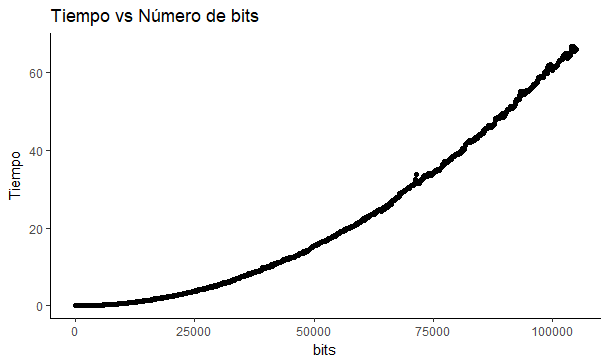
\includegraphics[width=0.5\textwidth]{result1}
    \caption{Multiplicación de dos números a y b con la misma cantidad de bits}
    \label{fig:result1}
\end{figure}

 
En la imagen \ref{fig:result2-s} se muestra el tiempo vs el número de bits de dos números a y b a multiplicar con a $>$ b cuando a número tiene un largo de bits cambiante y b tiene un largo de bits fijo de  $2^100-1$, el número cambiante tiene el largo de bits que aparece en el eje x. Los números a multiplicar fueron generados aleatoriamente según su número de bits. 

\begin{figure}[!h]
    \centering
    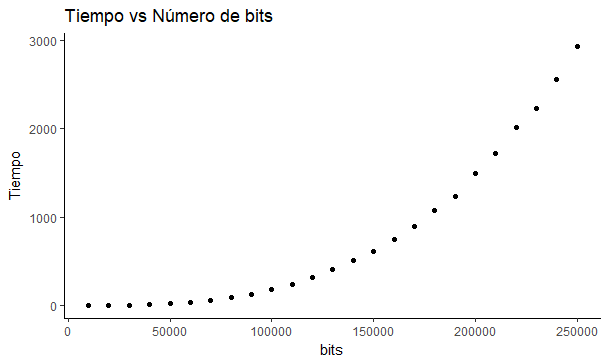
\includegraphics[width=0.45\textwidth]{result2-s}
    \caption{Multiplicación de dos números a$\cdot$b con a $>$ b,  a es fijo y b variante}
    \label{fig:result2-s}
\end{figure}

Los datos con lo que se creo el gráfico \ref{fig:result2-s} se muestran en la tabla \ref{tab:result2-s}.

\begin{table}[h]
\centering
\caption{Resultados de multiplicar dos números a$\cdot$b con a $>$ b, a fijo y b variante}
\label{tab:result2-s}
\begin{tabular}{|l|l|}
\hline
N° bits & Tiempo (seg) \\ \hline
10000  & 0.266831    \\ \hline
20000  & 1.749454    \\ \hline
30000  & 5.307608    \\ \hline
40000  & 12.194655   \\ \hline
50000  & 23.345639   \\ \hline
60000  & 39.947685   \\ \hline
70000  & 62.885600   \\ \hline
80000  & 92.826035   \\ \hline
90000  & 131.680444  \\ \hline
100000 & 180.657729  \\ \hline
110000 & 244.533478  \\ \hline
120000 & 319.893299  \\ \hline
130000 & 408.241408  \\ \hline
140000 & 515.545736  \\ \hline
150000 & 619.613212  \\ \hline
160000 & 751.622437  \\ \hline
170000 & 899.317050  \\ \hline
180000 & 1080.881010 \\ \hline
190000 & 1238.962152 \\ \hline
200000 & 1493.745582 \\ \hline
210000 & 1717.450705 \\ \hline
220000 & 2014.780954 \\ \hline
230000 & 2233.099756 \\ \hline
240000 & 2563.618059 \\ \hline
250000 & 2937.357255 \\ \hline
\end{tabular}
\end{table}

En la imagen \ref{fig:result2-s} se muestra el tiempo vs el número de bits de dos números a y b a multiplicar con a $>$ b cuando b número tiene un largo de bits cambiante y a tiene un largo de bits fijo de  $2^{100}-1$, el número cambiante tiene el largo de bits que aparece en el eje x. Los números a multiplicar fueron generados aleatoriamente según su número de bits.


\begin{figure}[!h]
    \centering
    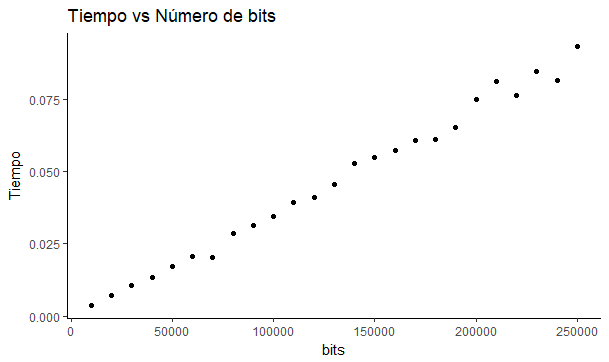
\includegraphics[width=0.45\textwidth]{result3}
    \caption{Multiplicación de dos números dos números a$\cdot$b con a $>$ b, a variante y b fijo}
    \label{fig:result3}
\end{figure}


La tabla con la que se creo el gráfico \ref{fig:result3} se muestran en la tabla \ref{tab:result3}.


\begin{table}[h]
\centering
\caption{Resultados de multiplicar dos números aleatorios de dos números a$\cdot$b con a $>$ b,  a fijo y b variante}
\label{tab:result3}
\begin{tabular}{|l|l|}
\hline
N° bits & Tiempo (seg) \\ \hline
10000  & 0.003576 \\ \hline
20000  & 0.007298 \\ \hline
30000  & 0.010669 \\ \hline
40000  & 0.013326 \\ \hline
50000  & 0.017059 \\ \hline
60000  & 0.020606 \\ \hline
70000  & 0.020369 \\ \hline
80000  & 0.028653 \\ \hline
90000  & 0.031274 \\ \hline
100000 & 0.034317 \\ \hline
110000 & 0.039210 \\ \hline
120000 & 0.041115 \\ \hline
130000 & 0.045586 \\ \hline
140000 & 0.052769 \\ \hline
150000 & 0.055029 \\ \hline
160000 & 0.057380 \\ \hline
170000 & 0.060642 \\ \hline
180000 & 0.061165 \\ \hline
190000 & 0.065194 \\ \hline
200000 & 0.074877 \\ \hline
210000 & 0.081134 \\ \hline
220000 & 0.076351 \\ \hline
230000 & 0.084789 \\ \hline
240000 & 0.081468 \\ \hline
250000 & 0.093469 \\ \hline
\end{tabular}
\end{table}

\section{Conclusiones}

Los resultados demuestran que efectivamente la complejidad de la multiplicación rusa es $\mathcal{O}(n \log (n))$, esto se puede ver claramente en la forma de la curva de la figura \ref{fig:result1}.

Además de que la rapidez de multiplicación depende únicamente de la cantidad de bits del número que va a ser divido en dos, esto se comprueba en la figura \ref{fig:result2-s} versus la figura \ref{fig:result3}, en la primera el número a dividir con un largo variante de que va desde $2^{10000}-1$ bits hasta $2^{250000}-1$, en cambio en la segunda figura se dejo el número a dividir como un número  $2^{100}-1$ bits, logrando que en el segundo experimento tuviera un notablemente menor tiempo de ejecución al tener siempre una cantidad fija de 100 iteraciones, por lo que es conveniente a la hora de multiplicar dos números $a\cdot b$ siempre dividir por dos el menor número y multiplicar por dos el mayor, aunque esto implique quedarse sin memoria más rápido debido a que el segundo número puede alcanzar un límite de memoria más temprano.
\\\\
Por último a pesar de que existen mejores algoritmos para multiplicar números grandes como Karatsuba, la multiplicación rusa se presenta como un método interesante a la hora de multiplicar dos números y sirve mucho cuando se debe considerar un número en su forma binaria, también sirve para trabajar números grandes usando lápiz y papel de manera más rápida y simple ya que reemplaza las típicas tablas de multiplicar con dos operaciones simples como son el multiplicar por dos y el dividir por dos.
\\\\
En definitiva, lo que en principio puede parecer una operación tan fácil como lo es multiplicar, puede convertirse en algo tan difícil y largo como un trabajo de investigación, y a pesar de que algunas formas de multiplicar pretendan facilitar la multiplicación, la hacen más compleja.

\nocite{AS00}

\nocite{KPR86}

\nocite{ISO/IEC9899}

\renewcommand\refname{Bibliography}

\bibliographystyle{plainnat} % or try abbrvnat or unsrtnat
\bibliography{bi} % refers to example.bib
%\printbibliography

%-----------------------------------------------//

\onecolumn 

\appendix

\section*{Apéndice A: Multiplicación rusa en C}

\begin{minted}{c}
#define I(a) (a - '0')
#define MAX 100000000

void russianmul(char * a, char * b, char * result) {
  //Declaración  de variables
  int la = strlen(a);
  int lb = strlen(b);
  char * aux = (char * ) malloc(la + 1);
  char * aux2 = (char * ) malloc(lb + MAX + 1);
  char * aux3 = (char * ) malloc((la + lb) + MAX);

  memset(result, '0', la + lb);
  result[0] = '\0';

  //Ciclo Multiplicación rusa
  while (a[0]) { //Mientras a no sea 0
    if (I(a[strlen(a) - 1]) % 2) { //si a es impar
      longsum(b, result, aux3); //Se suma el primer segundo número por el resultado
      strcpy(result, aux3);
    }
    longdiv(a, aux); //se divide el primer número por 2
    strcpy(a, aux);
    longmulti(b, aux2); //Se multiplica el segundo número por dos
    strcpy(b, aux2);
  }

  //Liberación memoria
  free(aux);
  free(aux2);
  free(aux3);
}
\end{minted}


\section*{Apéndice B: División por 2 dígito a dígito en C}

\begin{minted}{c}
#define I(a) (a - '0')
#define MAX 100000000

void longdiv(char *a, char *c){
    int la = strlen(a);
    memset(c, '0', la);
    c[la] = '\0';
    int carry = 0;
    int n=0;
    int i;
    for(i=0; i<la; i=i+1){
        n = (carry*10 + I(a[i]))/2; 
        carry = (carry*10 + I(a[i])) - 2*n;
        c[i] = n + '0';
    }
    if(c[0] == '0'){ //se elimina el cero que quede adelante
  			 memmove(c, c + 1, la);
  	     c[la] = '\0';
    }

}
\end{minted}

\section*{Apéndice C: Multiplicación por 2 dígito a dígito en C}

\begin{minted}{c}
#define I(a) (a - '0')
#define MAX 100000000

void longmulti(const char *a, char *c){
	int i = 0, k = 0, carry, n, la;

	la = strlen(a);
	memset(c, '0', la + 1);
	c[la + 2] = '\0';
	for (i = la - 1, k = i + 1; i >= 0; i--){
		n = I(a[i]) * 2 + I(c[k]);
		carry = n / 10;
		c[k] = (n % 10) + '0';
		k--;
		c[k] += carry;
	}

	if(c[0] == '0'){
		memmove(c, c + 1, la);
		c[la] = '\0';
     }
}
\end{minted}

\section*{Apéndice D: Suma clásica de dos enteros en C}

\begin{minted}{c}
#define I(a) (a - '0')
#define MAX 100000000


void longsum(const char * a,  const char * b, char * c){
  int la = strlen(a);
  int lb = strlen(b);
  int carry = 0;
  int sum;
  memset(c, '0', la+1); //llena c de 0
	//Crea un arreglo aux con el mismo largo que a
    //pero con los valores de b y lleno adelante con ceros
	char *aux= (char *)malloc(la+2);
	memset(aux, '0', la-lb);
    aux[la-lb] = '\0';
	strcat(aux,b);
  while( la >  0) {
      sum = I(a[la-1]) + I(aux[la-1]) + carry; // se suman dos digitos más el carry
      carry = sum/10; //si es mayor a 10 el carry es zero
      c[la] = sum%10 + '0'; // se guarda el primer digito de la suma como resultado
      la--;
  }
	if (carry >0) { //si la última suma es mayor a 10 entonces
		c[0] = carry + '0';
	}
	la = lb = strlen(a);
  if(c[0] == '0'){ //se eliminan los ceros de adelante
      memmove(c, c + 1, la);
       c[la] = '\0';
     }
    free(aux);
}
\end{minted}



\end{document}


